\begin{frame}
  \frametitle{Cíle práce a úvod do problematiky}
  \small
  \begin{block}{Cíle práce}
    \begin{itemize}
      \item Seznámit se s kvantově inspirovanými optimalizačními algoritmy
      \item Vybrat a implementovat různé algoritmy z vybrané třídy
      \item Navrhnout a realizovat experimenty na vybraném optimalizačním problému
      \item Porovnat kvantové algoritmy mezi sebou i s klasickými metodami
      \item Provést srovnávací analýzu a vyhodnotit výsledky
    \end{itemize}
  \end{block}

  \begin{block}{Úvod do problematiky}
    \begin{itemize}
      \item Kvantově inspirované algoritmy nacházejí podněty v \emph{kvantové mechanice}.
      \item Nabízejí potenciál pro efektivní řešení složitých úloh.
      \item Byla vybrána třída: \textit{Quantum Inspired Evolutionary Algorithms (QIEA)}.
    \end{itemize}
  \end{block}
\end{frame}



\begin{frame}
  \frametitle{Způsob řešení}
  \begin{columns}
    \column{0.5\textwidth}
    \small
    \textbf{Evoluční algoritmy (EA)} nacházejí inspiraci v~biologické evoluci:
      \begin{itemize}      
        \item standardně reprezentace jedinců bitovými či číselnými řetězci,
        \item evoluce skrze operátory selekce, rekombinace a mutace,
      \end{itemize}

    \vspace{3.5em}

    \begin{block}{}
    \IncMargin{1em}
    \begin{algorithm}[H]
      \scriptsize
      \SetAlCapFnt{\scriptsize}
      \SetAlCapNameFnt{\scriptsize}
      \caption{Schéma obecného EA}
      \SetAlgoLined
      \emph{Inicializace} a \emph{ohodnocení} počáteční populace\;
      \While{není splněna ukončující podmínka}{
        \emph{Selekce} rodičů a jejich \emph{rekombinace}\;
        \emph{Mutace} vzniklých potomků\;
        \emph{Ohodnocení} nově vzniklých jedinců\;
        \emph{Selekce} jedinců do nové populace\;
      }
    \end{algorithm}
    \end{block}

    \column{0.5\textwidth}
    \small
    \textbf{Kvantově inspirované EA} rozšiřují EA o~koncepty z kvantové mechaniky:
    \begin{itemize}
        \item kvantová reprezentace jedinců \emph{qubity}:
        \begin{equation*}
          \begin{bmatrix}
            \alpha_1 & \alpha_2 & \dots & \alpha_m \\
            \beta_1  & \beta_2  & \dots & \beta_m
          \end{bmatrix}
          \text{, kde } \alpha^2_i + \beta^2_i = 1
        \end{equation*}
        \item evoluce skrze kvantové operátory,
        \item měření pro získání klasických řešení.
    \end{itemize}
    

    \begin{block}{}
    \IncMargin{1em}
    \begin{algorithm}[H]
      \scriptsize
      \SetAlCapFnt{\scriptsize}
      \SetAlCapNameFnt{\scriptsize}
      \caption{Schéma obecného QIEA}
      \SetAlgoLined
        \emph{Inicializace} kvantové populace\;
        \While{není splněna ukončující podmínka}{
        \emph{Měření} kvantové populace\;
        \emph{Ohodnocení} klasické populace\;
        \emph{Aktualizace} kvantových stavů kvantovými operátory\;
      }
      \end{algorithm}
    \end{block}
  \end{columns}
\end{frame}



\begin{frame}
  \frametitle{Zvolené kvantově inspirované evoluční algoritmy}
  \small
  \begin{columns}
    \column{0.68\textwidth}
      \begin{enumerate}
        \item \textbf{Kvantově inspirovaný genetický algoritmus}\\(\textit{Quantum Inspired Genetic Algorithm\,--\,QIGA})~\cite{qiga}:
        \begin{itemize}
          \item vliv nejlepšího nalezeného řešení.
        \end{itemize}
        \item \textbf{Kvantově inspirované simulované žíhání}\\(\textit{Quantum-Inspired Simulated Annealing\,--\,QISA})~\cite{qisa}:
        \begin{itemize}
          \item pravděpodobnost ovlivněna teplotou.
        \end{itemize}
        \item \textbf{Kvantová evoluce roje}\\(\textit{Quantum Swarm Evolutionary\,--\,QSE})~\cite{qse}:
        \begin{itemize}
          \item kvantový stav reprezentován kvantovým úhlem.
        \end{itemize}
        \item \textbf{Kvantově inspirovaná optimalizace rojem částic}\\(\textit{Quantum-Inspired Particle Swarm Optimization\,--\,QIPSO}): 
        \begin{itemize}
          \item jedná se o \emph{vlastní návrh}.
        \end{itemize}
      \end{enumerate}
    \column{0.34\textwidth}
    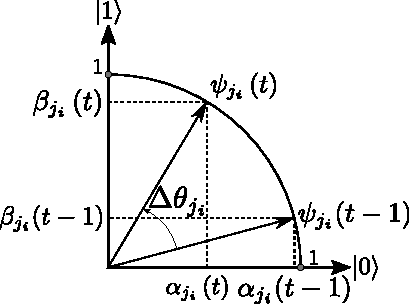
\includegraphics[width=\textwidth]{img/qiga-rotation-gate.pdf}
    {
      \vspace{0.5em}
      \scriptsize
      \centering
      \emph{Obrázek 1:} Kvantové rotační hradlo~\cite{qisa}.
    }
  \end{columns}
\end{frame}

\begin{frame}
  \frametitle{Pseudokód QIPSO}
  \IncMargin{1.5em}
  \begin{algorithm}[H]
    \scriptsize
    \SetAlCapFnt{\scriptsize}
    \SetAlCapNameFnt{\scriptsize}
    \caption{Kvantově inspirovaná optimalizace rojem částic}
    $t \gets 0$\;
    Inicializace populace $Q\left(t\right)$ kvantových chromozomů\;
    Inicializace počátečních rychlostí $V\left(t\right)$\;
    Inicializace nejlepších řešení populace $B\left(t\right)$ a globálně nejlepších řešení $G\left(t\right)$\;
    \While{$t < t_{\text{max}}$}{
        $t \gets t + 1$\;
        Vytvoření množiny řešení $P\left(t\right)$ pozorováním populace $Q\left(t-1\right)$\;
        \uIf{\emph{Nejlepší řešení z} $P\left(t\right)$ $>$ $B\left(t-1\right)$}{
            Uložení nejlepších řešení z $P\left(t\right)$ do $B\left(t\right)$\;
        }
        \Else{
            Uložení $B\left(t-1\right)$ do $B\left(t\right)$\;
        }
        \uIf{\emph{Nejlepší řešení z} $B\left(t\right)$ $>$ $G\left(t-1\right)$}{
            Uložení nejlepšího řešení z $B\left(t\right)$ do $G\left(t\right)$\;
        }
        \Else{
            Uložení $G\left(t-1\right)$ do $G\left(t\right)$\;
        }
        Vytvoření $V\left(t\right)$ pomocí $B\left(t\right)$ a $G\left(t\right)$ vzorcem: $v_{j_i}\left(t\right) \leftarrow \omega \cdot v_{j_i}\left(t-1\right) + c_1 \cdot r_1 \cdot (b_{j_i}\left(t\right) - p_{j_i}\left(t\right)) + c_2 \cdot r_2 \cdot (g_i\left(t\right) - p_{j_i}\left(t\right))$\;
        Vytvoření $Q\left(t\right)$ pomocí $V\left(t\right)$ aplikací kvantového rotačního hradla\;
    }
  \end{algorithm}
\end{frame}

\begin{frame}
  \frametitle{Návrh experimentů}
  \small
  \begin{block}{Optimalizační problém}
    \begin{itemize}
      \item Varianta 0-1 \emph{problému batohu} řešená na instancích různých velikostí.
    \end{itemize}
  \end{block}

  \begin{block}{Ladění parametrů}
    \begin{itemize}
      \item Provedeno na instancích se 100, 250 a 500 položkami.
      \item U každého algoritmu byly vybrány nejlepší parametry.
    \end{itemize}
  \end{block}

  \begin{block}{Hlavní experimenty}
    \begin{itemize}
      \item Spuštěno na instancích se 1\,000, 2\,000, 5\,000 a 10\,000 položkami.
      \item Použita odladěná konfigurace každého algoritmu.
      \item Každý experiment: 30 nezávislých běhů, 10\,000 (a také 100\,000) evaluací.
    \end{itemize}
  \end{block}
\end{frame}


\begin{frame}
  \frametitle{Srovnání \emph{QIEA} při 10\,000 evaluacích}
    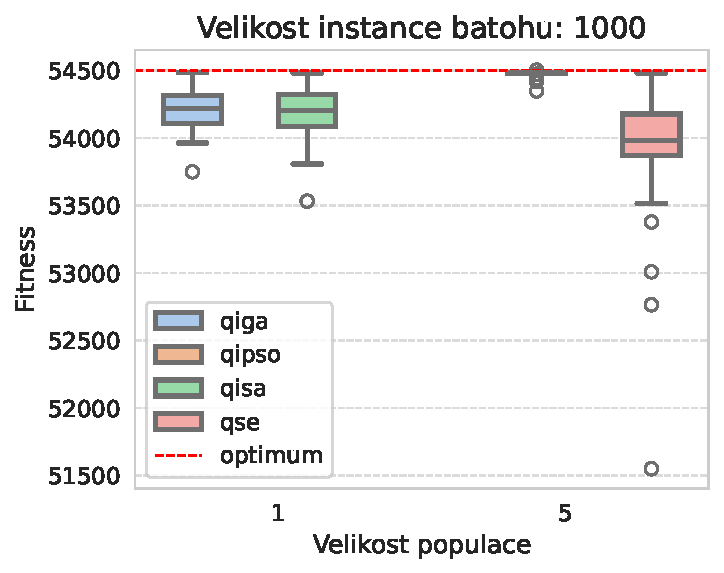
\includegraphics[width=0.32\textwidth]{img/10000/best_all_qiea_1000.pdf}
    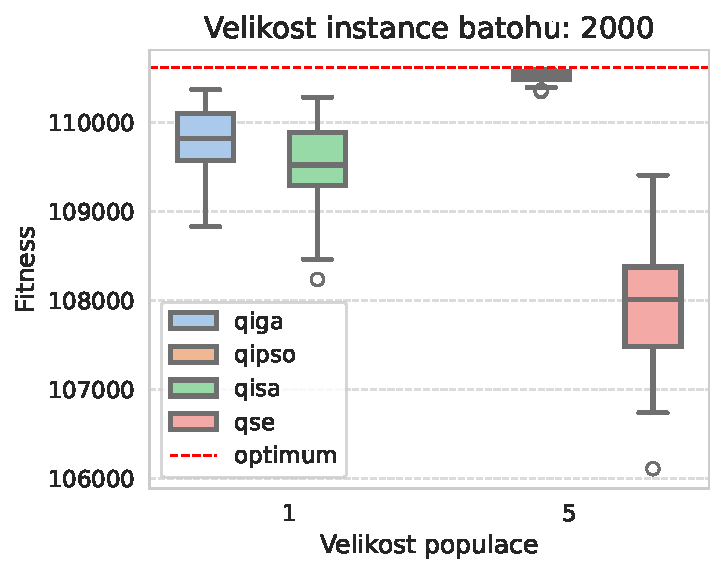
\includegraphics[width=0.32\textwidth]{img/10000/best_all_qiea_2000.pdf}
    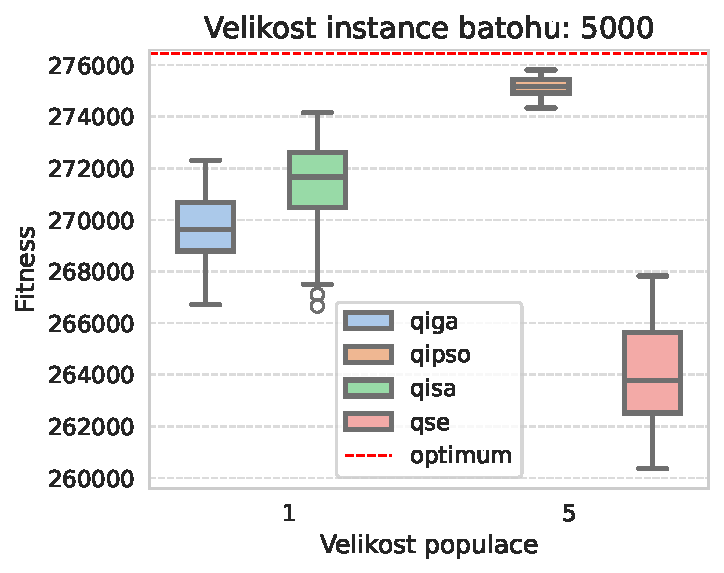
\includegraphics[width=0.32\textwidth]{img/10000/best_all_qiea_5000.pdf}

    \vspace{0.5em}
    \scriptsize
    \centering
    \emph{Obrázek 2:} Data prezentovaná na grafu byla získána na instancích problému batohu 1\,000, 2\,000 a 5\,000 pomocí 30 nezávislých běhů s 10\,000 evaluacemi na běh.
\end{frame}

\begin{frame}
  \frametitle{Srovnání \emph{QIEA} při 10\,000 evaluacích}
  \begin{columns}
    \column{0.48\textwidth}
      \centering
      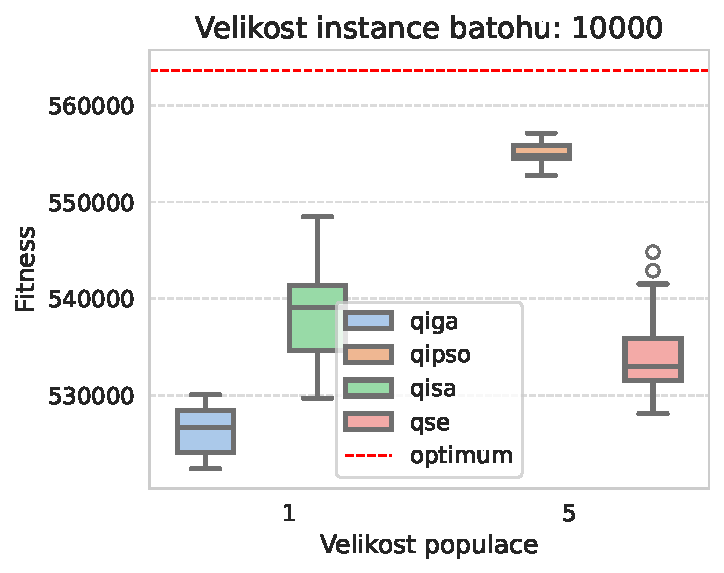
\includegraphics[width=\linewidth]{img/10000/best_all_qiea_10000.pdf}

      \vspace{0.5em}
      \scriptsize
      \centering
      \emph{Obrázek 3}: Data prezentovaná na grafu byla získána na instanci problému batohu velikosti 10\,000, pomocí 30 nezávislých běhů s 10\,000 evaluacemi na běh.
    \column{0.52\textwidth}
    \footnotesize
    \begin{tabular}{lcccc}
      \toprule
      \multirow{2}{*}{\textbf{Algoritmus}} &
      \multicolumn{4}{c}{\textbf{Instance}} \\
      & \textbf{1\,000} & \textbf{2\,000} & \textbf{5\,000} & \textbf{10\,000} \\
      \midrule
      QIGA  & 54\,485 & 110\,373 & 272\,306 & 530\,066 \\[1ex]
      QISA  & 54\,481 & 110\,287 & 274\,150 & 548\,460 \\[1ex]
      QSE   & 54\,481 & 108\,387 & 267\,827 & 544\,824 \\[1ex]
      QIPSO & \textbf{54\,503} & \textbf{110\,592} & \textbf{275\,805} & \textbf{557\,120} \\
      \midrule
      Optimum & 54\,503 & 110\,625 & 276\,457 & 563\,647 \\
      \bottomrule
    \end{tabular}

    \vspace{0.5em}
    \scriptsize
    \centering
    \emph{Tabulka 1:} Nejlepší dosažené fitness hodnoty jednotlivými kvantově inspirovanými evolučními algoritmy.
  \end{columns}
\end{frame}

\begin{frame}
  \frametitle{Srovnání \emph{QIEA} při 100\,000 evaluacích}
  \begin{columns}
    \column{0.48\textwidth}
      \centering
      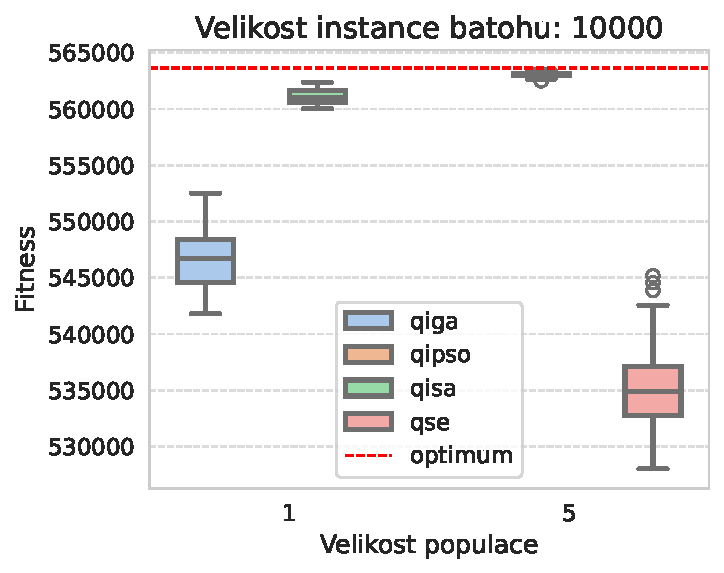
\includegraphics[width=\linewidth]{img/100000/best_all_qiea_10000.pdf}

      \vspace{0.5em}
      \scriptsize
      \centering
      \emph{Obrázek 4:} Data prezentovaná na grafu byla získána na instanci problému batohu velikosti 10\,000, pomocí 30 nezávislých běhů s 100\,000 evaluacemi na běh.
    \column{0.52\textwidth}
      \centering
      \footnotesize
      \begin{tabular}{l c}
                \toprule
          \textbf{Algoritmus} & \textbf{Maximální fitness} \\
          \midrule
          QIGA    & 552\,513 \\[1ex]
          QISA    & 562\,368 \\[1ex]
          QSE     & 545\,171 \\[1ex]
          QIPSO   & \textbf{563\,464} \\
          \midrule
          Optimum & 563\,647 \\
          \bottomrule
      \end{tabular}

      \vspace{0.5em}
      \scriptsize
      \centering
      \emph{Tabulka 2:} Nejlepší dosažené fitness hodnoty jednotlivými kvantově inspirovanými evolučními algoritmy.
  \end{columns}
\end{frame}

\begin{frame}
  \footnotesize
  \frametitle{Srovnání \emph{QIEA} s klasickými optimalizačními algoritmy~\cite{cmp}}
  \centering
  \begin{tabular}{c c c c c}
    \toprule
    \multirow{2}{*}{\textbf{Algoritmus}} &
    \multicolumn{4}{c}{\textbf{Instance}} \\
          & 1\,000  & 2\,000   & 5\,000   & 10\,000 \\
    \midrule
    SA    & 36\,179 &  65\,793 & 150\,731 & \textbf{563\,647} \\[1ex]
    GA    &     130 & 102\,340 & 102\,340 & 562\,556 \\[1ex]
    GSA   & 14\,927 &  25\,579 &  49\,306 & 292\,225 \\[1ex]
    DP    & \textbf{54\,503} & \textbf{110\,625} & \textbf{276\,457} & 106\,464 \\[1ex]
    BB    & 53\,397 & 109\,679 & 275\,720 &      130 \\
    \midrule
    QIGA  & 54\,485 & 110\,373 & 272\,306 & 552\,513 \\[1ex]
    QISA  & 54\,481 & 110\,287 & 274\,150 & 562\,368 \\[1ex]
    QSE   & 54\,481 & 108\,387 & 267\,827 & 545\,171 \\[1ex]
    QIPSO & \textbf{54\,503} & 110\,592 & 275\,805 & 563\,464 \\
    \midrule
    Optimum & 54\,503 & 110\,625 & 276\,457 & 563\,647 \\
    \bottomrule
  \end{tabular}

  \vspace{1em}
  \scriptsize
  \emph{Tabulka 3:} Nejlepší dosažené fitness hodnoty jednotlivými algoritmy.

  \vspace{0.5em}
  \tiny
  \begin{center}
    \emph{Poznámka:}
    SA\,--\,Simulated Annealing,
    GA\,--\,Genetic Algorithm,
    GSA\,--\,Greedy Search Algorithm,
    DP\,--\,Dynamic Programming,
    BB\,--\,Branch and Bound.
  \end{center}
\end{frame}

\begin{frame}
  \frametitle{Děkuji za pozornost}
  \begin{columns}
    \column{0.48\textwidth}
      \centering
      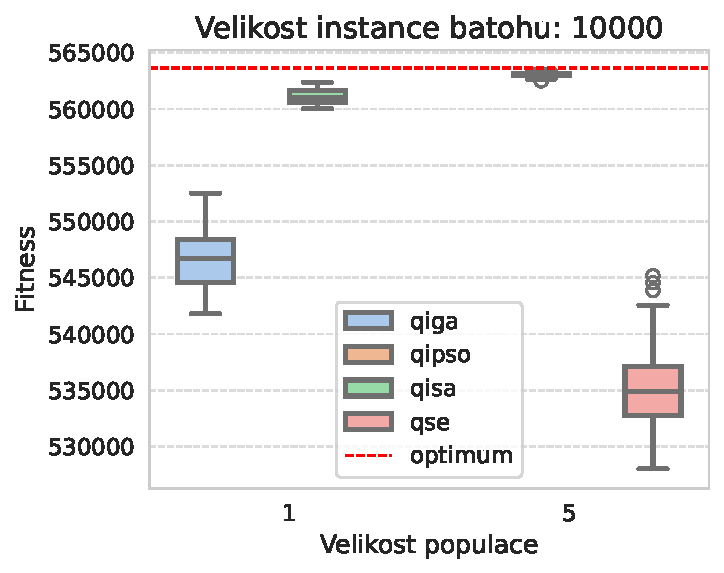
\includegraphics[width=0.9\linewidth]{img/100000/best_all_qiea_10000.pdf}

      \vspace{0.5em}
      \scriptsize
      \centering
      \emph{Obrázek:} Data prezentovaná na grafu byla získána na instanci problému batohu velikosti 10\,000, pomocí 30 nezávislých běhů s 100\,000 evaluacemi na běh.
    \column{0.52\textwidth}
      \footnotesize
      \begin{tabular}{lcccc}
        \toprule
        \multirow{2}{*}{\textbf{Algoritmus}} &
        \multicolumn{4}{c}{\textbf{Instance}} \\
        & \textbf{1\,000} & \textbf{2\,000} & \textbf{5\,000} & \textbf{10\,000} \\
        \midrule
        QIGA  & 54\,485 & 110\,373 & 272\,306 & 530\,066 \\[1ex]
        QISA  & 54\,481 & 110\,287 & 274\,150 & 548\,460 \\[1ex]
        QSE   & 54\,481 & 108\,387 & 267\,827 & 544\,824 \\[1ex]
        QIPSO & \textbf{54\,503} & \textbf{110\,592} & \textbf{275\,805} & \textbf{557\,120} \\
        \midrule
        Optimum & 54\,503 & 110\,625 & 276\,457 & 563\,647 \\
        \bottomrule
      \end{tabular}

      \vspace{0.5em}
      \scriptsize
      \centering
      \emph{Tabulka:} Nejlepší dosažené fitness hodnoty jednotlivými kvantově inspirovanými evolučními algoritmy při 10\,000 evaluacích.
  \end{columns}
  \begin{center}
    \vspace{1em}
    Výsledky této práce byly oceněny odborným panelem v rámci 
\includegraphics[width=0.18\linewidth]{img/ExcelAtFIT-logo.pdf}.  
  \end{center}
\end{frame}

\appendix{}
\begin{frame}
  \frametitle{Literatura}
    \bibliographystyle{bib-styles/Pysny/czplain}
    \scriptsize
    \begin{thebibliography}{9}
      \bibitem{qiga}
        Han, K.-H. a Kim, J.-H. 
        Quantum-inspired evolutionary algorithm for a class of combinatorial optimization. 
        \textit{IEEE Transactions on Evolutionary Computation} online. 1. vyd., 2002, sv. 6, č. 6, s. 580--593. ISSN 1941-0026. 
        Dostupné z: \url{https://doi.org/10.1109/TEVC.2002.804320}. [cit. 2025-06-22].

      \bibitem{qisa}
        Chen, Z. a Luo, P. 
        QISA: Incorporating quantum computation into Simulated Annealing for optimization problems. 
        In: IEEE. \textit{2011 IEEE Congress of Evolutionary Computation (CEC)} online. Institute of Electrical and Electronics Engineers, 2011 s. 2480--2487. ISBN 978-1-4244-7835-4. 
        Dostupné z: \url{https://doi.org/10.1109/CEC.2011.5949925}. [cit. 2025-06-22].

      \bibitem{qse}
        Wang, Y.; Feng, X.-Y.; Huang, Y.-X.; Pu, D.-B.; Zhou, W.-G. et al. 
        A novel quantum swarm evolutionary algorithm and its applications. 
        \textit{Neurocomputing} online. 1. vyd., 2007, sv. 70, č. 4, s. 633--640. ISSN 0925-2312. 
        Dostupné z: \url{https://doi.org/https://doi.org/10.1016/j.neucom.2006.10.001}. [cit. 2025-06-22].

    
      \bibitem{cmp} 
        Ezugwu, A. E.; Pillay, V.; Hirasen, D.; Sivanarain, K. a Govender, M. 
        A Comparative Study of Meta-Heuristic Optimization Algorithms for 0\,--\,1 Knapsack Problem: Some Initial Results. 
        \textit{IEEE Access} online. 1. vyd., 2019, sv. 7, č. 1, s. 43979--44001. 
        Dostupné z: \url{https://doi.org/10.1109/ACCESS.2019.2908489}. [cit. 2025-06-22].
      \end{thebibliography}      
\end{frame}
